\documentclass[]{tufte-handout}

% ams
\usepackage{amssymb,amsmath}

\usepackage{ifxetex,ifluatex}
\usepackage{fixltx2e} % provides \textsubscript
\ifnum 0\ifxetex 1\fi\ifluatex 1\fi=0 % if pdftex
  \usepackage[T1]{fontenc}
  \usepackage[utf8]{inputenc}
\else % if luatex or xelatex
  \makeatletter
  \@ifpackageloaded{fontspec}{}{\usepackage{fontspec}}
  \makeatother
  \defaultfontfeatures{Ligatures=TeX,Scale=MatchLowercase}
  \makeatletter
  \@ifpackageloaded{soul}{
     \renewcommand\allcapsspacing[1]{{\addfontfeature{LetterSpace=15}#1}}
     \renewcommand\smallcapsspacing[1]{{\addfontfeature{LetterSpace=10}#1}}
   }{}
  \makeatother

\fi

% graphix
\usepackage{graphicx}
\setkeys{Gin}{width=\linewidth,totalheight=\textheight,keepaspectratio}

% booktabs
\usepackage{booktabs}

% url
\usepackage{url}

% hyperref
\usepackage{hyperref}

% units.
\usepackage{units}


\setcounter{secnumdepth}{-1}

% citations
\usepackage{natbib}
\bibliographystyle{plainnat}

% pandoc syntax highlighting
\usepackage{color}
\usepackage{fancyvrb}
\newcommand{\VerbBar}{|}
\newcommand{\VERB}{\Verb[commandchars=\\\{\}]}
\DefineVerbatimEnvironment{Highlighting}{Verbatim}{commandchars=\\\{\}}
% Add ',fontsize=\small' for more characters per line
\newenvironment{Shaded}{}{}
\newcommand{\KeywordTok}[1]{\textcolor[rgb]{0.00,0.44,0.13}{\textbf{#1}}}
\newcommand{\DataTypeTok}[1]{\textcolor[rgb]{0.56,0.13,0.00}{#1}}
\newcommand{\DecValTok}[1]{\textcolor[rgb]{0.25,0.63,0.44}{#1}}
\newcommand{\BaseNTok}[1]{\textcolor[rgb]{0.25,0.63,0.44}{#1}}
\newcommand{\FloatTok}[1]{\textcolor[rgb]{0.25,0.63,0.44}{#1}}
\newcommand{\ConstantTok}[1]{\textcolor[rgb]{0.53,0.00,0.00}{#1}}
\newcommand{\CharTok}[1]{\textcolor[rgb]{0.25,0.44,0.63}{#1}}
\newcommand{\SpecialCharTok}[1]{\textcolor[rgb]{0.25,0.44,0.63}{#1}}
\newcommand{\StringTok}[1]{\textcolor[rgb]{0.25,0.44,0.63}{#1}}
\newcommand{\VerbatimStringTok}[1]{\textcolor[rgb]{0.25,0.44,0.63}{#1}}
\newcommand{\SpecialStringTok}[1]{\textcolor[rgb]{0.73,0.40,0.53}{#1}}
\newcommand{\ImportTok}[1]{#1}
\newcommand{\CommentTok}[1]{\textcolor[rgb]{0.38,0.63,0.69}{\textit{#1}}}
\newcommand{\DocumentationTok}[1]{\textcolor[rgb]{0.73,0.13,0.13}{\textit{#1}}}
\newcommand{\AnnotationTok}[1]{\textcolor[rgb]{0.38,0.63,0.69}{\textbf{\textit{#1}}}}
\newcommand{\CommentVarTok}[1]{\textcolor[rgb]{0.38,0.63,0.69}{\textbf{\textit{#1}}}}
\newcommand{\OtherTok}[1]{\textcolor[rgb]{0.00,0.44,0.13}{#1}}
\newcommand{\FunctionTok}[1]{\textcolor[rgb]{0.02,0.16,0.49}{#1}}
\newcommand{\VariableTok}[1]{\textcolor[rgb]{0.10,0.09,0.49}{#1}}
\newcommand{\ControlFlowTok}[1]{\textcolor[rgb]{0.00,0.44,0.13}{\textbf{#1}}}
\newcommand{\OperatorTok}[1]{\textcolor[rgb]{0.40,0.40,0.40}{#1}}
\newcommand{\BuiltInTok}[1]{#1}
\newcommand{\ExtensionTok}[1]{#1}
\newcommand{\PreprocessorTok}[1]{\textcolor[rgb]{0.74,0.48,0.00}{#1}}
\newcommand{\AttributeTok}[1]{\textcolor[rgb]{0.49,0.56,0.16}{#1}}
\newcommand{\RegionMarkerTok}[1]{#1}
\newcommand{\InformationTok}[1]{\textcolor[rgb]{0.38,0.63,0.69}{\textbf{\textit{#1}}}}
\newcommand{\WarningTok}[1]{\textcolor[rgb]{0.38,0.63,0.69}{\textbf{\textit{#1}}}}
\newcommand{\AlertTok}[1]{\textcolor[rgb]{1.00,0.00,0.00}{\textbf{#1}}}
\newcommand{\ErrorTok}[1]{\textcolor[rgb]{1.00,0.00,0.00}{\textbf{#1}}}
\newcommand{\NormalTok}[1]{#1}

% longtable

% multiplecol
\usepackage{multicol}

% strikeout
\usepackage[normalem]{ulem}

% morefloats
\usepackage{morefloats}


% tightlist macro required by pandoc >= 1.14
\providecommand{\tightlist}{%
  \setlength{\itemsep}{0pt}\setlength{\parskip}{0pt}}

% title / author / date
\title{Data Science Unplugged: Additive Boosting}
\author{Brent Johnson}
\date{2018-01-19}


\begin{document}

\maketitle




\subsection{Data Science Unplugged}\label{data-science-unplugged}

\begin{marginfigure}
You can easily \href{http://www.centralmoment.com}{download} the R
Mardown version of this document and reproduce all my examples on your
own. You may just need to install the rpart and rpart.plot packages.
\end{marginfigure}

When I want to really understand a machine learning or statistical tool,
to really get a feel for how it works, I like to step away from the
finished package and code the algorithm by hand. Sure, once in
production mode I will use a package. Package authors often include
helpful options and features that aren't worth my time to reconstruct.
Finished packages are often optimized for speed. But to truly understand
the nuts and bolts of what these packages are doing, I often need to
first step away from them. I often like to code these algorithms in base
R, Pandas (Python), or SAS/IML. Doing so forces me to understand exactly
how the machine learning tool works.

In this document I'll explore additive boosting. As I do so, I'm going
to tie my hands, so to speak, and just use base R as much as possible.
As far as ground rules go, I will allow myself the use of plotting
packages, the \href{https://www.tidyverse.org/}{tidyverse}, and other
packages as long as they don't mask the fundamental algorithm that I'm
trying most to make clear.

The benefits of this manual approach include not only an understanding
of the algorithm, but greater knowledge of its assumptions and when it
is or isn't likely to work well. Doing so also gives me great ideas for
further improving the algorithm, possibly inventing unique enhancements
on my own.

\subsection{Boosting and ensemble predictive
models}\label{boosting-and-ensemble-predictive-models}

There are multiple flavors of boosting.
\href{http://blog.kaggle.com/2017/01/23/a-kaggle-master-explains-gradient-boosting/}{Gradient
boosting}, for example, is a current favorite over at
\href{https://www.kaggle.com/competitions}{Kaggle}. In this document,
I'll explore the slightly older additive boosting cousin--called
AdaBoost. Readers wanting to learn more ought to pursue Schapire and
Freund's
\href{https://www.amazon.com/Boosting-Foundations-Algorithms-Adaptive-Computation/dp/0262526034}{excellent
book}.

All boosting algorithms follow an
\href{https://en.wikipedia.org/wiki/Ensemble_learning}{ensemble
modeling} approach to generating predictions. Ensemble models are used
almost exclusively for prediction (a limitation or caveat that I'll get
to later) and generate their predictions only after averaging over
dozens or hundreds (i.e., an ensemble) of separate ingredient models or
predictions. Ensemble models algorithms are meta-models, in sense.
They're ``models of models.''

\subsection{Setting Things Up}\label{setting-things-up}

I first need some dummy data to which I can apply my homegrown AdaBoost
algorithm. The below generates the dummy data used extensively by Ryan
Tibshirini and described in one of his
\href{http://www.stat.cmu.edu/~ryantibs/datamining/lectures/25-boost.pdf}{lectures
on page 8} and in Chapter 10 of the excellent book,
\href{https://www.amazon.com/Elements-Statistical-Learning-Prediction-Statistics/dp/0387848576}{The
Elements of Statistical Learning}. The following chunk generates a data
frame, \texttt{X}, containing ten normally distributed independent
random variables or predictors. I also generate a binary dependent
variable, \texttt{Y}, that's only loosely correlated with the predictor
variables:

\begin{marginfigure}
Many AdaBoost implimentations require a binary outcome variable be coded
as -1 or 1. My example requires 0 or 1 coded outcomes.
\end{marginfigure}

\begin{Shaded}
\begin{Highlighting}[]
\KeywordTok{set.seed}\NormalTok{(}\DecValTok{415}\NormalTok{)}
\NormalTok{X <-}\StringTok{ }\KeywordTok{data.frame}\NormalTok{(}\KeywordTok{matrix}\NormalTok{(}\KeywordTok{rnorm}\NormalTok{(}\DecValTok{10} \OperatorTok{*}\StringTok{ }\DecValTok{1000}\NormalTok{, }\DecValTok{0}\NormalTok{, }\DecValTok{1}\NormalTok{), }
    \DataTypeTok{ncol =} \DecValTok{10}\NormalTok{))}
\NormalTok{X}\OperatorTok{$}\NormalTok{Y <-}\StringTok{ }\KeywordTok{ifelse}\NormalTok{(}\KeywordTok{rowSums}\NormalTok{(}\KeywordTok{data.frame}\NormalTok{(}\KeywordTok{lapply}\NormalTok{(X, }\ControlFlowTok{function}\NormalTok{(x) x}\OperatorTok{^}\DecValTok{2}\NormalTok{))) }\OperatorTok{>}\StringTok{ }
\StringTok{    }\KeywordTok{qchisq}\NormalTok{(}\FloatTok{0.5}\NormalTok{, }\DecValTok{10}\NormalTok{), }\DecValTok{1}\NormalTok{, }\DecValTok{0}\NormalTok{)}
\end{Highlighting}
\end{Shaded}

The above data will support my development of a ``weak learner''--a
classification that, on its own, enables an only slightly
better-than-chance prediction. In words, my \texttt{Y} variable is built
from the sum of my 10 squared independent variables. If the sum exceeds
the median of a chi-square distribution having 10 degrees of freedom
(which yields a value of 9.3), then \texttt{Y=1}; otherwise \texttt{Y=0}
In general, boosting algorithms show the greatest prediction success
when applied using a weak learner like this one. Further below in this
article I'll contrast this with both a strong learner and even a learner
containing just random noise.

I'm working in R, so, to further prepare my work environment I need to
load some libraries. I first load rpart, a package for fitting
\href{https://cran.r-project.org/web/packages/rpart/vignettes/longintro.pdf}{classification
and regression trees} and also rattle and rpart.plot which is helpful
for generating nice plots of classification trees like those rpart
produces.

\begin{Shaded}
\begin{Highlighting}[]
\KeywordTok{library}\NormalTok{(rpart)}
\KeywordTok{library}\NormalTok{(rattle)}
\KeywordTok{library}\NormalTok{(rpart.plot)}
\end{Highlighting}
\end{Shaded}

So, right at the start here I'm assuming the reader is somewhat familiar
with
\href{https://www.amazon.com/Classification-Regression-Wadsworth-Statistics-Probability/dp/0412048418}{classification
via decision or regression trees} and I won't code a classification tree
from scratch in base R. That would be exhausting and detract from my
purpose here. For what it's worth, I could just as easily demonstrate
boosting if I employed logistic regression instead of a classification
tree. Also, one can apply boosting to standard linear regression models
as well as to classification trees. But boosting appears to be most
often applied in tree-based settings, so I'll stick with rpart.

\begin{marginfigure}
As an experiment, the reader could create a boosted logistic regression
by inserting the code, ``model \textless{}- glm(Y \textasciitilde{} X1 +
X2 + X3 + X4 + + X5 + X6 + X7 + X8 + X9 + X10, weights=weight, data=X,
family=`quasibinomial')'' in place of the rpart function below. Just
recall, however, that the predicted values from such a model are on the
logistic scale. So, one would need to modify the predict() function
accordingly in order to append the 0/1 predicted values to
yhat{[}{[}i{]}{]}.
\end{marginfigure}

\subsection{Boosting described in words--and in simple
code}\label{boosting-described-in-wordsand-in-simple-code}

AdaBoost is perhaps the simplest boosting algorithm. Following Schapire
and Freund's
\href{https://www.amazon.com/Boosting-Foundations-Algorithms-Adaptive-Computation/dp/0262526034}{excellent
description}, AdaBoost consists of the following steps:

\begin{enumerate}
\def\labelenumi{\arabic{enumi}.}
\tightlist
\item
  Fit a model to one's data
\item
  Compute the predicted outcome
\item
  Increase the relative weight given to the poorly predicted
  observations; reduce the relative weight given to successfully
  predicted outcomes.
\item
  Wash, rinse, and repeat for n iterations, saving the predicted
  outcomes from each iteration
\item
  Compute the winning prediction using a weighted average of the
  predictions from the n iterations
\end{enumerate}

I implement these steps in the following code chunks. This is the
AdaBoost algorithm unplugged. I begin by initializing a few objects for
collecting the results. And I initialize a weight variable. This weight
variable starts of with identical values for each observation or record
in \texttt{X}.

\begin{Shaded}
\begin{Highlighting}[]
\CommentTok{# create placeholders for the forecast}
\CommentTok{# ensemble}
\NormalTok{alpha <-}\StringTok{ }\KeywordTok{vector}\NormalTok{(}\StringTok{"list"}\NormalTok{)}
\NormalTok{yhat <-}\StringTok{ }\KeywordTok{vector}\NormalTok{(}\StringTok{"list"}\NormalTok{)}
\NormalTok{models <-}\StringTok{ }\KeywordTok{list}\NormalTok{()}
\NormalTok{success.vec <-}\StringTok{ }\KeywordTok{mean}\NormalTok{(X}\OperatorTok{$}\NormalTok{Y)}

\NormalTok{X}\OperatorTok{$}\NormalTok{weight <-}\StringTok{ }\DecValTok{1}\OperatorTok{/}\KeywordTok{nrow}\NormalTok{(X)  }\CommentTok{# Intitialize a weight vector}
\end{Highlighting}
\end{Shaded}

I next code AdaBoost. I first specify the number of boosted trees or
iterations (\texttt{niter}) that I want in my ensemble. I then
repeatedly estimate a classification tree (using the rpart function),
saving the predicted values from each member of the ensemble into
\texttt{yhat}. As for the construction of my classification tree and the
rpart options, I won't go into a deep explanation. The function options
below merely specify that each tree in my ensemble contains a single
split with a minimum size of 100 observations per split. A
classification or decision tree with a single split like this is called
a decision ``stump.''

The AdaBoost algorithm inside the loop below might be best understood by
working from the bottom up. Near the end of the algorithm, the final
predicted probability (\texttt{predicted.prob}) of each observation is a
weighted average of the predictions from all 100 trees or members of the
ensemble. The relative weight (\texttt{alpha.weight}) given each
ingredient prediction is determined by \texttt{alpha}. And the
\texttt{alpha} for each tree is in turn constructed from each model's
logged relative prediction error (\texttt{.5*log((1-error)/error)}. Note
that this prediction error is simply 1 minus the sum of the weights for
all successfully predicted outcomes
(\texttt{1-\ sum(as.numeric(X\$Y\ ==\ yhat{[}{[}i{]}{]})*X\$weight)}).

By experimenting with different \texttt{error} values one can see that
an ingredient tree's prediction is given exponentially more weight the
higher its prediction success. For example, if a tree predicts no better
than chance (error = .5) then its alpha would be zero. Conversely if a
given tree in the ensemble predicts with 100\% success (error = 0) then
the weight given its prediction would be infinitely high (since
\texttt{.5*log((1-0)/0)\ =\ Inf}). This is an exponential loss function
and is the default option in many AdaBoost package implementations.
Following this rule, highly predictive models in the ensemble get
exponentially more weight than poorly predictive ones.

\begin{Shaded}
\begin{Highlighting}[]
\KeywordTok{set.seed}\NormalTok{(}\DecValTok{415}\NormalTok{)}
\NormalTok{niter <-}\StringTok{ }\DecValTok{100}

\ControlFlowTok{for}\NormalTok{ (i }\ControlFlowTok{in} \KeywordTok{seq}\NormalTok{(niter)) \{}
\NormalTok{    model <-}\StringTok{ }\KeywordTok{rpart}\NormalTok{(Y }\OperatorTok{~}\StringTok{ }\NormalTok{X1 }\OperatorTok{+}\StringTok{ }\NormalTok{X2 }\OperatorTok{+}\StringTok{ }\NormalTok{X3 }\OperatorTok{+}\StringTok{ }\NormalTok{X4 }\OperatorTok{+}\StringTok{ }\OperatorTok{+}\NormalTok{X5 }\OperatorTok{+}\StringTok{ }
\StringTok{        }\NormalTok{X6 }\OperatorTok{+}\StringTok{ }\NormalTok{X7 }\OperatorTok{+}\StringTok{ }\NormalTok{X8 }\OperatorTok{+}\StringTok{ }\NormalTok{X9 }\OperatorTok{+}\StringTok{ }\NormalTok{X10, }\DataTypeTok{data =}\NormalTok{ X, }\DataTypeTok{maxdepth =} \DecValTok{1}\NormalTok{, }
        \DataTypeTok{minbucket =} \DecValTok{100}\NormalTok{, }\DataTypeTok{cp =} \OperatorTok{-}\DecValTok{1}\NormalTok{, }\DataTypeTok{xval =} \DecValTok{0}\NormalTok{, }\DataTypeTok{weights =}\NormalTok{ weight, }
        \DataTypeTok{method =} \StringTok{"class"}\NormalTok{)}
\NormalTok{    models[[i]] <-}\StringTok{ }\NormalTok{model}
\NormalTok{    yhat[[i]] <-}\StringTok{ }\KeywordTok{ifelse}\NormalTok{(}\KeywordTok{predict}\NormalTok{(model)[, }\DecValTok{2}\NormalTok{] }\OperatorTok{>}\StringTok{ }
\StringTok{        }\FloatTok{0.5}\NormalTok{, }\DecValTok{1}\NormalTok{, }\DecValTok{0}\NormalTok{)}
\NormalTok{    error <-}\StringTok{ }\DecValTok{1} \OperatorTok{-}\StringTok{ }\KeywordTok{sum}\NormalTok{(}\KeywordTok{as.numeric}\NormalTok{(X}\OperatorTok{$}\NormalTok{Y }\OperatorTok{==}\StringTok{ }\NormalTok{yhat[[i]]) }\OperatorTok{*}\StringTok{ }
\StringTok{        }\NormalTok{X}\OperatorTok{$}\NormalTok{weight)}
\NormalTok{    alpha[[i]] <-}\StringTok{ }\FloatTok{0.5} \OperatorTok{*}\StringTok{ }\KeywordTok{log}\NormalTok{((}\DecValTok{1} \OperatorTok{-}\StringTok{ }\NormalTok{error)}\OperatorTok{/}\NormalTok{error)}
\NormalTok{    weight.adjustment <-}\StringTok{ }\KeywordTok{ifelse}\NormalTok{(yhat[[i]] }\OperatorTok{==}\StringTok{ }\NormalTok{X}\OperatorTok{$}\NormalTok{Y, }
        \KeywordTok{exp}\NormalTok{(}\OperatorTok{-}\NormalTok{alpha[[i]]), }\KeywordTok{exp}\NormalTok{(alpha[[i]]))}
\NormalTok{    new.unscaled.weight <-}\StringTok{ }\NormalTok{X}\OperatorTok{$}\NormalTok{weight }\OperatorTok{*}\StringTok{ }\NormalTok{weight.adjustment}
\NormalTok{    X}\OperatorTok{$}\NormalTok{weight <-}\StringTok{ }\NormalTok{new.unscaled.weight}\OperatorTok{/}\KeywordTok{sum}\NormalTok{(new.unscaled.weight)}
    
    \CommentTok{# create weights for combining iterations in}
    \CommentTok{# the ensemble}
\NormalTok{    alpha.weight <-}\StringTok{ }\KeywordTok{lapply}\NormalTok{(alpha, }\ControlFlowTok{function}\NormalTok{(x) x}\OperatorTok{/}\KeywordTok{sum}\NormalTok{(}\KeywordTok{unlist}\NormalTok{(alpha)))}
    
    \CommentTok{# created a weighted predicted probability}
    \CommentTok{# from the ensemble, weighted by alpha}
\NormalTok{    predicted.prob <-}\StringTok{ }\KeywordTok{rowSums}\NormalTok{(}\KeywordTok{data.frame}\NormalTok{(}\KeywordTok{Map}\NormalTok{(}\StringTok{"*"}\NormalTok{, }
\NormalTok{        yhat, alpha.weight)))}
    
    \CommentTok{# assign prediction outcome}
\NormalTok{    predicted <-}\StringTok{ }\KeywordTok{ifelse}\NormalTok{(predicted.prob }\OperatorTok{>}\StringTok{ }\FloatTok{0.5}\NormalTok{, }
        \DecValTok{1}\NormalTok{, }\DecValTok{0}\NormalTok{)}
    
    \CommentTok{# record the success progress}
\NormalTok{    success.rate <-}\StringTok{ }\KeywordTok{sum}\NormalTok{(predicted }\OperatorTok{==}\StringTok{ }\NormalTok{X}\OperatorTok{$}\NormalTok{Y)}\OperatorTok{/}\KeywordTok{nrow}\NormalTok{(X)}
\NormalTok{    success.vec <-}\StringTok{ }\KeywordTok{c}\NormalTok{(success.vec, success.rate)}
\NormalTok{\}}
\end{Highlighting}
\end{Shaded}

The \texttt{alpha} term in the code above also informs the weights given
to each observation. On close inspection it should be clear that at each
iteration of the algorithm, the rows inside \texttt{X\$weight} that
correspond to correctly predicted values of \texttt{Y} receive less
relative weight. And weight values corresponding to incorrect
predictions receive greater relative weight. The change in observational
weights causes the rpart function to generate different classification
trees with each iteration. Each tree chases after those observations
that were erroneously predicted during the previous iteration.

\textbackslash{}begin\{marginfigure\}
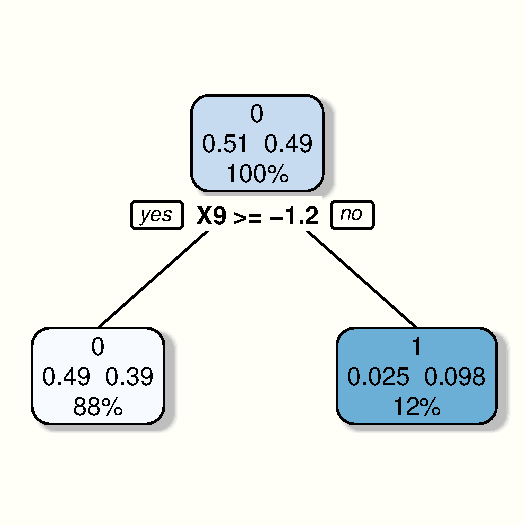
\includegraphics{2018-02-19-data-science-unplugged-additive-boosting_files/figure-latex/first.iteration-1}
\textbackslash{}caption{[}AdaBoost's first tree starts off with equal
weights{]}\{AdaBoost's first tree starts off with equal weights.
Predicted values of 0 for Y go to the left; Predicted values of 1 go to
the right. The true proportions are described inside the boxes, e.g.,
49\% of all \texttt{X\$Y} values are both predicted to equal zero and
have a true value of 0.\}\label{fig:first.iteration}
\textbackslash{}end\{marginfigure\} To make this clear, I plot the first
tree or iteration generated from the above AdaBoost example. This tree
splits on variable \texttt{X9}. That is, when starting with equal weight
given to all data records, the best variable for splitting successes and
failures is \texttt{X9}. In this iteration, the model predicts all
observations for which X9 \textgreater{}= -1.2 as failures (Y=0). This
makes up 88\% of the sample. And the model predicts all other
observations (the remaining 12\% of the sample) as successes (Y=1). The
error for this first iteration is 58.8\% (which is .49 + .098) which is
somewhat higher than chance prediction.

The second tree reflects a data frame wherein the observations with
poorly predicted values from the first iteration receive greater weight.
As a result, the highly weighted observations drive a different
classification tree--one that now splits on variable \texttt{X4}. In the
iterative loop above, this process continues for 98 more iterations. Our
AdaBoost ensemble has 100 total classification trees.

\begin{marginfigure}
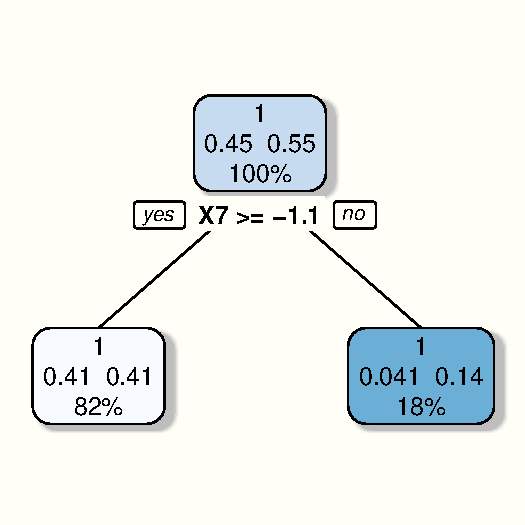
\includegraphics{2018-02-19-data-science-unplugged-additive-boosting_files/figure-latex/second.iteration-1} \caption[This is the tree from AdaBoost's second iteration]{This is the tree from AdaBoost's second iteration. In this tree and all subsequent trees, the weights differ across the observations and, so, the weighted proportion of correct (and incorrect) observations in each branch begins to change.}\label{fig:second.iteration}
\end{marginfigure}

It's easy to plot the progress and rate of success of the AdaBoost
algorithm as it completes the different iterations. In the next plot we
see that the algorithm starts off making successful predictions at a
rate somewhat better than chance. However, over subsequent iterations
the algorithm improves and the ensemble produces a successful prediction
for 85\% of the observations. That's pretty good for a model that
started with just weakly correlated predictor values. Predictions using
AdaBoost appear to be a great improvement over the single best-fitting
predictive stump with which we started.

\begin{marginfigure}
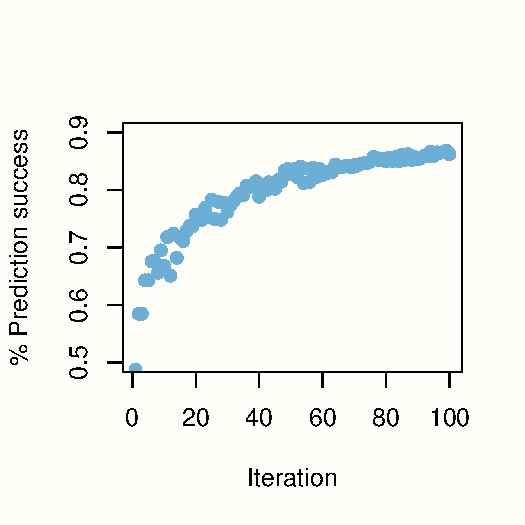
\includegraphics{2018-02-19-data-science-unplugged-additive-boosting_files/figure-latex/boost.plot.weak-1} \caption[Prediction success from AdaBoost applied to a WEAK learner]{Prediction success from AdaBoost applied to a WEAK learner. AdaBoost begins with a classificatation just slightly better than chance and gradually improves with more iterations.}\label{fig:boost.plot.weak}
\end{marginfigure}

It's also interesting to monitor AdaBoost's progress at successfully
predicting the individual observations of interest. In the next code
chunk below and in the object called \texttt{yhat.successes} I record
the occasions each record in my data frame was correctly predicted by an
AdaBoost tree. Recall that the object \texttt{yhat} that I initialized
at the beginning is a list object containing 100 vectors--one for each
tree in the example above. And each vector inside \texttt{yhat} contains
1000 values--one for each predicted value of \texttt{X\$Y}. The object
\texttt{yhat.successes} below, therefore, records which of AdaBoost
iterations successfully predicted each data record. And using
\texttt{head()} I display the prediction results for the first 6 such
observations (in rows) and the first 8 AdaBoost trees or iterations (in
columns). One can see that the first, fourth, and fifth observation in
this example were correctly predicted in the first classification tree
(\texttt{X1} column) but these same observations were then
unsuccessfully predicted in the second classification tree (\texttt{X2})
column. Over subsequent AdaBoost iterations, observations often
alternate between being successfully or unsuccessfully predicted as the
observation weights change and rpart selects different variables for
constructing the classification stump.

\begin{Shaded}
\begin{Highlighting}[]
\NormalTok{yhat.successes <-}\StringTok{ }\KeywordTok{sapply}\NormalTok{(yhat, }\ControlFlowTok{function}\NormalTok{(z) z }\OperatorTok{==}\StringTok{ }\NormalTok{X}\OperatorTok{$}\NormalTok{Y)}
\KeywordTok{head}\NormalTok{(}\KeywordTok{data.frame}\NormalTok{(yhat.successes)[,}\DecValTok{1}\OperatorTok{:}\DecValTok{8}\NormalTok{])}
\end{Highlighting}
\end{Shaded}

\begin{verbatim}
##      X1    X2    X3    X4    X5    X6    X7
## 1  TRUE FALSE  TRUE FALSE  TRUE FALSE  TRUE
## 2 FALSE  TRUE FALSE  TRUE  TRUE  TRUE FALSE
## 3 FALSE  TRUE FALSE  TRUE FALSE  TRUE FALSE
## 4  TRUE FALSE  TRUE FALSE  TRUE FALSE  TRUE
## 5  TRUE FALSE  TRUE FALSE  TRUE FALSE  TRUE
## 6 FALSE  TRUE FALSE  TRUE FALSE  TRUE FALSE
##      X8
## 1 FALSE
## 2  TRUE
## 3  TRUE
## 4 FALSE
## 5 FALSE
## 6  TRUE
\end{verbatim}

I note that there was no one single tree or iteration that correctly
predicted all or even anything close to 85\% of the observations. In
AdaBoost, some trees successfully predict some observations; other trees
successfully predict others. AdaBoost is an ensemble modeling method.
The final prediction rate is achieved by averaging over all 100 trees or
iterations in the ensemble. However, the code below confirms that 100\%
of the observations were correctly predicted \emph{at least once} over
the 100 iterations above.

\begin{Shaded}
\begin{Highlighting}[]
\NormalTok{success.pct <-}\StringTok{ }\KeywordTok{sum}\NormalTok{(}\KeywordTok{apply}\NormalTok{(yhat.successes, }\DecValTok{1}\NormalTok{, }\ControlFlowTok{function}\NormalTok{(z) }\KeywordTok{max}\NormalTok{(z))) }\OperatorTok{/}\StringTok{ }\KeywordTok{nrow}\NormalTok{(X) }
\NormalTok{success.pct}
\end{Highlighting}
\end{Shaded}

\begin{verbatim}
## [1] 1
\end{verbatim}

Now, I don't show the code for revealing it here, but in this simulated
data set, all observations were actually correctly predicted at least
once after only SIX AdaBoost iterations. However, I don't terminate
AdaBoost after just six iterations. The values of \texttt{alpha} for
combining the different tree predictions may not yet be optimized.
AdaBoost needs to return to the unsuccessfully predicted observations in
iteration number six and further refine their weights. Rules for
deciding when to terminate AdaBoost iterations should balance increased
prediction success (a greater number of AdaBoost iterations will improve
prediction) with over-fitting (too many iterations will result in a tree
ensemble that doesn't generalize well outside this particular data set).
Splitting one's data into training vs.~validation samples (or adopting a
\href{https://en.wikipedia.org/wiki/Cross-validation_(statistics)}{k-fold}
validation) is essential for tuning any boosting algorithm and for
determining the ideal number of AdaBoost iterations.

\subsection{When AdaBoost fails--Example
\#2}\label{when-adaboost-failsexample-2}

To understand the type of occasion when AdaBoost is likely to be most
useful, it is helpful to run AdaBoost on different simulated data
scenarios. Here below I revise the data generation process I used above.
I now create a dependent or outcome variable (\texttt{X\$Y}) such that
it's very easily classified by just one of the previously generated
independent variables (\texttt{X1}). The following code generates a
strong learner, a data frame containing a variable that very easily
predicts the outcome.

\begin{Shaded}
\begin{Highlighting}[]
\CommentTok{# Generate just one continuous strong learner}
\NormalTok{X}\OperatorTok{$}\NormalTok{pr =}\StringTok{ }\DecValTok{1}\OperatorTok{/}\NormalTok{(}\DecValTok{1}\OperatorTok{+}\KeywordTok{exp}\NormalTok{(}\OperatorTok{-}\NormalTok{X}\OperatorTok{$}\NormalTok{X1))         }\CommentTok{# pass X1 through an inv-logit function}
\NormalTok{X}\OperatorTok{$}\NormalTok{Y =}\StringTok{ }\KeywordTok{rbinom}\NormalTok{(}\DecValTok{1000}\NormalTok{,}\DecValTok{1}\NormalTok{,X}\OperatorTok{$}\NormalTok{pr)       }\CommentTok{# generate a bernoulli response variable}
\end{Highlighting}
\end{Shaded}

I then re-run the same AdaBoost algorithm above for 100 iterations. Here
to the right is the plot of its prediction success.

\begin{marginfigure}
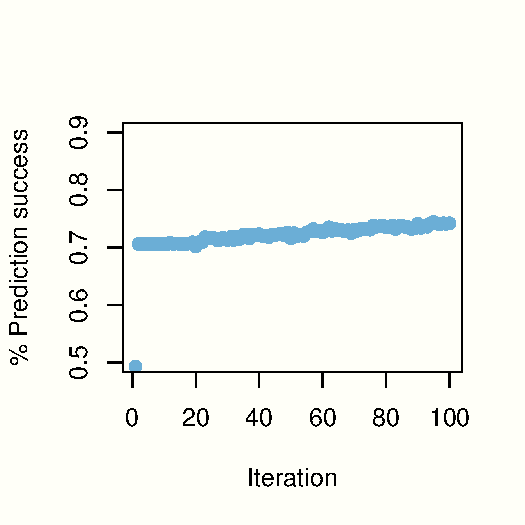
\includegraphics{2018-02-19-data-science-unplugged-additive-boosting_files/figure-latex/boost.plot.strong-1} \caption[Prediction success from AdaBoost using a STRONG learner]{Prediction success from AdaBoost using a STRONG learner. Here AdaBoost starts off predicting well but improvement is not as good as it is with the weak learner above.}\label{fig:boost.plot.strong}
\end{marginfigure}

Comparing this progress plot with the plot from the weak learner, it's
clear that AdaBoost's initial prediction success starts off much higher
when begun with a strong learner. However, prediction doesn't improve
nearly as quickly and appears to approach an asymptote that's much lower
than that for the weak learner. With the strong learner, AdaBoost's
prediction success after 100 iterations approaches around 73\%. By
contrast, with the weak learner above, the prediction success approaches
85\%. This difference demonstrates one of AdaBoost's key strengths.
AdaBoost does better with a large number of loosely predictive variables
than it does with just a few strongly predictive ones With a great many
loosely predictive variables such as in this example, AdaBoost has more
opportunity to adjust the weights, to allow different predictor
variables to define the stump, and to improve model fit.

\subsection{Pushing the limits of AdaBoost--Example
\#3}\label{pushing-the-limits-of-adaboostexample-3}

Boosting works best when fed with a weak learner like in the first
example. However, here's something interesting: AdaBoost will also
\emph{appear} to improve prediction even when presented with a learner
that's less than weak. To show this, I next simulate the application of
AdaBoost on a ``noise learner.'' In the code below, I define
\texttt{X\$Y} as completely independent of any of the predictor
variables. Here \texttt{X\$Y} is now simply the outcome of 1,000 random
Bernoulli trials:

\begin{Shaded}
\begin{Highlighting}[]
\CommentTok{# Generate a random dependent variable}
\KeywordTok{set.seed}\NormalTok{(}\DecValTok{5}\NormalTok{)}
\NormalTok{X}\OperatorTok{$}\NormalTok{Y =}\StringTok{ }\KeywordTok{rbinom}\NormalTok{(}\DecValTok{1000}\NormalTok{,}\DecValTok{1}\NormalTok{,.}\DecValTok{5}\NormalTok{)      }\CommentTok{# bernoulli response variable}
\end{Highlighting}
\end{Shaded}

Let's run AdaBoost one more time on the noise data above and plot its
progress:

\begin{marginfigure}
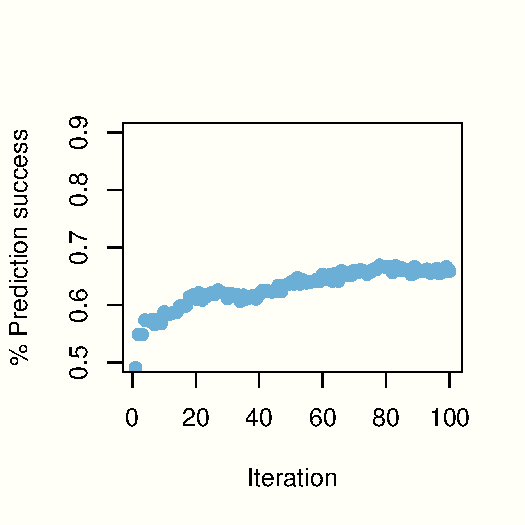
\includegraphics{2018-02-19-data-science-unplugged-additive-boosting_files/figure-latex/boost.plot.noise-1} \caption[Prediction success from AdaBoost and a NOISE learner]{Prediction success from AdaBoost and a NOISE learner. Even with noise data, AdaBoost improves prediction above chance after 100 iterations.}\label{fig:boost.plot.noise}
\end{marginfigure}

Wow! Even when tasked with predicting random noise, AdaBoost finds
better-than-chance prediction success. In this plot to the right, after
100 iterations AdaBoost correctly predicts over 65\% of the
observations. And if I were to run AdaBoost indefinitely and well beyond
100 iterations, AdaBoost's prediction success would gradually continue,
eventually growing towards 100\%. AdaBoost is truly adaptive. It's so
good at generating a predictive ensemble that, if allowed to run long
enough, it can find predictive gold even when there is none!

\subsection{Conslusions for boosting}\label{conslusions-for-boosting}

This highlights yet more strengths and weaknesses of AdaBoost as a
prediction algorithm. AdaBoost can take a mere weak learner and, via
adapting the data weights, find prediction success from an ensemble far
in excess of what one could achieve from a single classification tree
alone. That's a plus. It's ideal if one's task is to make predictions
given a collection of only loosely predictive independent variables. For
example, perhaps one is trying to predict, say, whether a potential oil
well contains enough oil to merit extraction. Assume in addition that
the seismic data one would normally use for predicting extraction
success, while fundamentally accurate and unbiased, is beset with
measurement error and background noise. AdaBoost might predict well in
such a situation.

But the lesson from the noise learner example should be to never
generalize a boosting algorithm's prediction success from a test sample
alone. As shown in Example \#3, one can achieve prediction success from
one's test sample even if the predictor variables bear no (unweighted)
relationship with the dependent variable. If I tried to apply the
results here to make predictions from an entirely new data set, I would
likely fail miserably. Boosting is prone to over-fitting. One ought to
employ cross-validation methods to reduce the risk of wrong
generalizations.

My second concern with AdaBoost--and this holds for all ensemble models
that I'm aware of--is that while it might be excellent at prediction,
AdaBoost is bad at story telling. What I mean is, it's very difficult to
interpret the results of a predictive ensemble. It's hard to tell
exactly which variables are most helpful in prediction. Granted, some
boosting implementations such as
\href{https://cran.r-project.org/web/packages/ada/ada.pdf}{ada} for R or
\href{https://github.com/scikit-learn/scikit-learn}{sklearn} for Python
include functions for displaying variable importance. Quite often,

\begin{quote}
``The measures are based on the number of times a variable is selected
for splitting, weighted by the squared improvement to the model as a
result of each split, and averaged over all trees''\\
\href{http://onlinelibrary.wiley.com/doi/10.1111/j.1365-2656.2008.01390.x/full}{Elith,
Leathwick, and Hastie (2008)}.
\end{quote}

That sounds intuitive and is indeed helpful. But this doesn't say
anything about which cut points or categories of an independent variable
make for the most accurate predictions. There's no summary about a
variable's predictive direction--whether increases or decreases in a
particular independent variable are generally associated with a positive
or negative outcome. In fact, it's entirely possible for a variable's
cut-point to change or its predictive direction to reverse over the
course of an ensemble's iterations if AdaBoost's weights change enough.
And it's not clear to me whether the variables and splits chosen for
their predictive performance near the end of the iterations (when the
data weights are more extreme and the effective sample size is less)
ought to be ranked just as highly as variables and splits selected
earlier in the ensemble when the observations are more equality
weighted. So, it's hard to tell an intuitive story to a client or one's
boss describing exactly which independent variables are most
predictive--and how they affect prediction.

Stepping back, I think it's helpful to consider the different purposes
or objectives for building machine learning models and to evaluate
AdaBoost in that context. Researchers implement machine learning
models--including additive boosting--for
\href{https://www.dezyre.com/article/types-of-analytics-descriptive-predictive-prescriptive-analytics/209}{a
variety of purposes}. And it's important to match one's algorithm with
one's modeling purpose. Some machine learning models are built to better
understand or describe the world. This is referred to as ``descriptive
modeling.'' Yet other models are built to help guide or optimize
decision making. These models attempt to tell the research what he or
she \emph{should} do. Models for economic policy making come to mind
here and are often built for this purpose. These models are called
``prescriptive'' or ``normative models''. Finally, researchers often
build models where the main purpose is simply prediction success. These
are referred to as ``predictive models''. I find AdaBoost and other
ensemble models most helpful when the goal is focused on predictive
performance and if one doesn't need to tell a detailed story around
which of the independent variables contribute (or how they contribute)
to the prediction. It's less helpful for other purposes. In this
context, a cross-validated AdaBoost model is a helpful modeling
framework and a valuable addition to the predictive modelers toolkit.

\bibliography{skeleton.bib}



\end{document}
